\documentclass[10pt,a4paper]{article}
\usepackage[left=1.5cm,right=1.5cm,top=1.5cm,bottom=1.5cm]{geometry}
\usepackage[utf8]{inputenc}
\usepackage[german]{babel}
\usepackage{amsmath}
\usepackage{amsfonts}
\usepackage{amssymb}
\usepackage{amsthm}
\usepackage{graphicx}

\newenvironment{packed_enum}{
\begin{enumerate}
  \setlength{\itemsep}{1pt}
  \setlength{\parskip}{0pt}
  \setlength{\parsep}{0pt}
}{\end{enumerate}}
\newcommand{\abs}[1]{\ensuremath{\left\vert#1\right\vert}}
\begin{document}
\section{Allgemeines}
\subsection{Nabla Operator $\nabla$}
\[
\vec{\nabla} = \left(\frac{\partial}{\partial x_1}, ..., \frac{\partial}{\partial x_n} \right)
\,\,\,\,\,\,\,\,\,\,\,\,\,\,\,\,\,\,\,\,\,\,\,\,\,\,\,\,
\vec{\nabla} \vec{V} = \sum\limits_{i=1}^n \frac{\partial V_i}{\partial x_i}
\]

\section{Partielle Differentialgleichungen}
\subsection{Homogene lineare partielle Differentialgleichungen 1. Ordnung}
\begin{packed_enum}
\item Umstellen in Normalform: $\sum\limits_{i = 1}^n a_i(\vec{x}) \cdot u_i = 0$, weitere Beispiele für $n=2$.
\item Charakteristische DGLs sind zu lösen: $\dot{x}(t) = a_1(x(t), y(t)); \dot{y}(t) = a_2(x(t), y(t))$
\begin{packed_enum}
\item Dabei darf man alle Gleichungen z.B. durch eine andere teilen
\item Hat man dies getan, erhält man z.B. $\dot{x}(t)=1$ und somit $x(t)=t+c$
\item $c=0$ kann zulaessig sein wenn Anfangswert gegeben ist, also $x=t$ in diesem Fall
\end{packed_enum}
\item Eine der Gleichungen durch Variablen der anderen darstellen: $y = \psi(x, C)$, nach $C(\vec{c})$ umstellen $C(\vec{c}) = \phi(x,y)$
\item $\Phi(\phi(x,y))$ mit beliebigem $\Phi$ aus $C^1$ ist die Lösung
\item Allgemein: $u(\vec{x}) = \Phi(\phi_1({x}), ... , \phi_{n-1}(\vec{x}))$
\end{packed_enum}

\subsection{Quasilineare partielle inhomogene Differentialgleichungen 1. Ordnung}
So sieht sie aus: $\sum\limits_{i=1}^n a_i(\vec{x}, u)\cdot u_{x_i} = b(\vec{x}, u)$

Lösen mit erweiterter quasilinearer homogener DGL: $\left( \sum\limits_{i=1}^n a_i(\vec{x}, u)\cdot U_{x_i} \right) + b(\vec{x}, u)\cdot U_u = 0$

Dann wie homogene lineare partielle Differentialgleichungen 1. Ordnung lösen.

Dann $U = 0$, Nach dem Satz über implizite Funktionen ergibt sich:

Zum Schluss eine Basis als Funktion der anderen Basis darstellen, nach $u$ umformen und $\psi(...)$ passend aussuchen.

Wir erhalten als allgemeine Loesung eine implizite Gleichung mit beliebige $C^1$ Funktion $\Phi$.	

\subsection{Anfangswertaufgaben}
$u(\vec{x}) = \Phi(\phi_1({x}), ... , \phi_{n-1}(\vec{x}))$

Anfangsfunktion: $u_0(s) := u(x(s), y(s))$ auf der Kurve $c(s) := (x(s), y(s))^T$.

\subsection{Burgersgleichung}
TODO

\subsection{Lineare inhomogene partielle Differentialgleichungen 2. Ordnung}
\[
\sum\limits_{i,j=1}^n a_{ij}(\vec{x})u_{x_ix_j} + \sum\limits_{i=1}^n b_i(\vec{x}) u_{x_i} + f(\vec{x})u = g(\vec{x})
\]

Für $n=2$ und $\vec{x}=(x,y)$: $au_{xx} +2bu_{xy}+cu_{yy} + du_x+eu_y+fu=g$

Matrix: $
\left(
\begin{matrix}
a & b \\
b & c \\
\end{matrix}
\right)
TODO$

elliptisch: Alle $\lambda_i \neq 0$ gleiches Vorzeichen

parabolisch: $\exists k : \lambda_k = 0$

hyperbolisch: $\exists! i : \lambda_i$ hat verschiedenes Vorzeichen von allen anderen $\lambda$.

ultrahyperbolisch: erst ab n=4: alle anderen Faelle

Wenn det:$
\begin{matrix}
> 0: \mbox{ elliptisch\ \ \ \ \ } \\
= 0: \mbox{ parabolisch\ } \\
< 0: \mbox{ hyperbolisch} \\
\end{matrix}
$

Für $n=2$ immer det nehmen, ultrahyperbolisch gibts nur in höheren Dimensionen.

Für $n=3$ nach einer spalte/zeile entwickeln und det(Rest) nehmen. Produkt der EW ist det, reicht aus.

3 Dim: $au_{xx}+2bu_{xy}+2cu_{xz}+2du_{yz}+eu_{yy}+fu_{zz}+gu_x +hu_y+iu_z+ju=k$

$\nabla^T
\begin{pmatrix}
a & b&c \\
b & e&d \\
c&d&f\\
\end{pmatrix}
\nabla u+\left(g - \nabla^T \begin{pmatrix}
a\\b\\c\\
\end{pmatrix}, h - \nabla^T \begin{pmatrix}
b\\e\\d\\
\end{pmatrix},i - \nabla^T \begin{pmatrix}
e\\d\\f\\
\end{pmatrix}\right)\nabla u + ju = k$

\subsubsection{Wärmeleitungsgleichung}
So sieht sie aus: $v_t = v_{xx} + g(x)$ mit einer beliebigen $C^1$ Funktion $g(x)$. $v_h(x,t)$ löst $0 = v_t - v_{xx}$.

Löse nun homogene Gleichung mit inhomogener Anfangsbedingung: Fourier! :)
\[v_h(x,t) = \sum\limits_{k=1}^{\infty} b_k \cdot sin\left(\frac{k \pi x}{z} \right) e^{-\frac{t k^2 \pi^2}{z^2}}
\,\,\,\,\,\,\,\,\,\,\,\,\,
T=2\cdot z
\,\,\,\,\,\,\,\,\,\,\,\,\,
b_k = \frac{2}{T} \int\limits_0^T f(x) \cdot sin\left( \frac{k \pi x}{z}\right) \mbox{ mit } f(x) = \mbox{ Anfangsbedingung}
\]

Koeffizientenvergleich d. Anfangsbedingung mit Summenansatz hilfreich!

Nun Inhomogenität lösen: Inhomogene Gleichung mit homogener Randbedingung und Anfangsbedingung: $\omega = \pi / z$

$v_p(x,t) \xrightarrow{Ansatz} v_p(x,t) = \sum\limits_{k=1}^{\infty} v_k(t) sin \left( k \omega x \right)$ und $v_k(0) = 0$.

In DGL einsetzen. $\sum\limits_{k=1}^{\infty} \left(\dot{v}_k(t) + k^2 \omega^2 v_k(t) \right) sin(k \omega x) = g(x)$
\pagebreak
\section{Polarkoordination}
\subsection{Produktansatz in Polarkoordinaten}
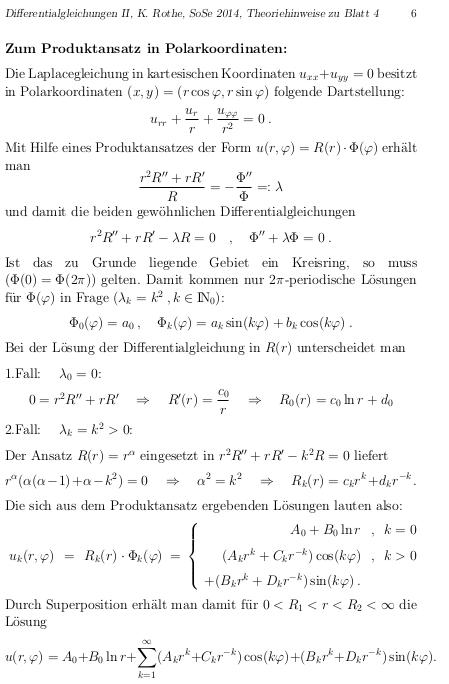
\includegraphics[scale=0.6]{ununderstandable}
\[
x = r\,cos\phi, y=r\,sin\phi \mbox{ mit } sin(2\phi)=2sin\phi cos\phi \mbox{ und } cos(3\phi)=4cos^3\phi - 3cos \phi
\]

TODO: Herleitung kann in der Klausur uebersprungen werden. Wegkuerzen!

\section{Dirichlet Problem}
Der Produktansatz $u(r, \phi) = R(r) \cdot \Phi(\phi)$ ergibt:
\begin{itemize}
\item
Kreis: $u(r, \phi) = A_0 + \sum\limits_{k=1}^\infty A_k r^k cos(k \phi) + B_k r^k sin(k \phi)$
\item
Halbkreis: $u(r, \phi) = \sum\limits_{k=1}^\infty A_k r^k sin(k \phi)$
\item
Kreisring: $u(r, \phi) = A_0 + B_0 ln|r| + \sum\limits_{k=1}^\infty \left(A_k r^k + C_k r^{-k} \right) cos(k \phi) + \left(B_k r^k + D_k r^{-k} \right) sin(k \phi)$
\item
Halbkreisring: $u(r, \phi) = \sum\limits_{k=1}^\infty \left(A_k r^k + C_k r^{-k} \right) sin(k \phi)$
\end{itemize}

Karthesischisierung: $x = cos(\phi)*r$, $y = r sin(\phi)$, $r = \sqrt{x^2 + y^2}$

$sin(\alpha \pm \beta) = sin(\alpha)\cdot cos(\beta) \pm sin(\beta)\cdot cos(\alpha)$ und $cos(\alpha \pm \beta) = cos(\alpha)\cdot cos(\beta) \mp sin(\alpha)\cdot sin(\beta)$

\section{d'Alembertsche Loesungsformel}
Fuer: $u_{tt} = c^2 u_{xx}$ ist $u(x,t) = \frac{1}{2}u_0(x+ct) + u_0(x-ct) + \frac{1}{6}\int\limits_{x-ct}^{x+ct} v_0\left(\xi\right) d \xi $

\end{document}
